% =====================================================================
%  FIGURES & TABLES TO PASTE  —  Group 41 report, Clarence's sections
%  Everything below is ready to copy straight into the report.
%
%  ONE-TIME SETUP (put near your other \usepackage lines, skip any you have):
%      \usepackage{graphicx}   % for the figure
%      \usepackage{booktabs}   % for \toprule \midrule \bottomrule
%      \usepackage{amssymb}    % only if \checkmark is undefined in the roles table
%
%  Also: upload architecture-two-projections.pdf into your Overleaf project.
%
%  HOW TO USE: each block has a "PASTE INTO ..." header telling you where it
%  goes, and an "IN-TEXT" note telling you what to write where the report
%  currently has a bare "Table 1" / "Figure 1" so the numbers auto-fill and
%  the List of Figures/Tables populate. Recompile twice.
% =====================================================================


% ####################################################################
% FIGURE 1  —  PASTE INTO §3.6  (near "...two projections (Figure 1)")
% IN-TEXT: replace "Figure 1" with   Figure~\ref{fig:arch}
% ####################################################################
\begin{figure}[t]
  \centering
  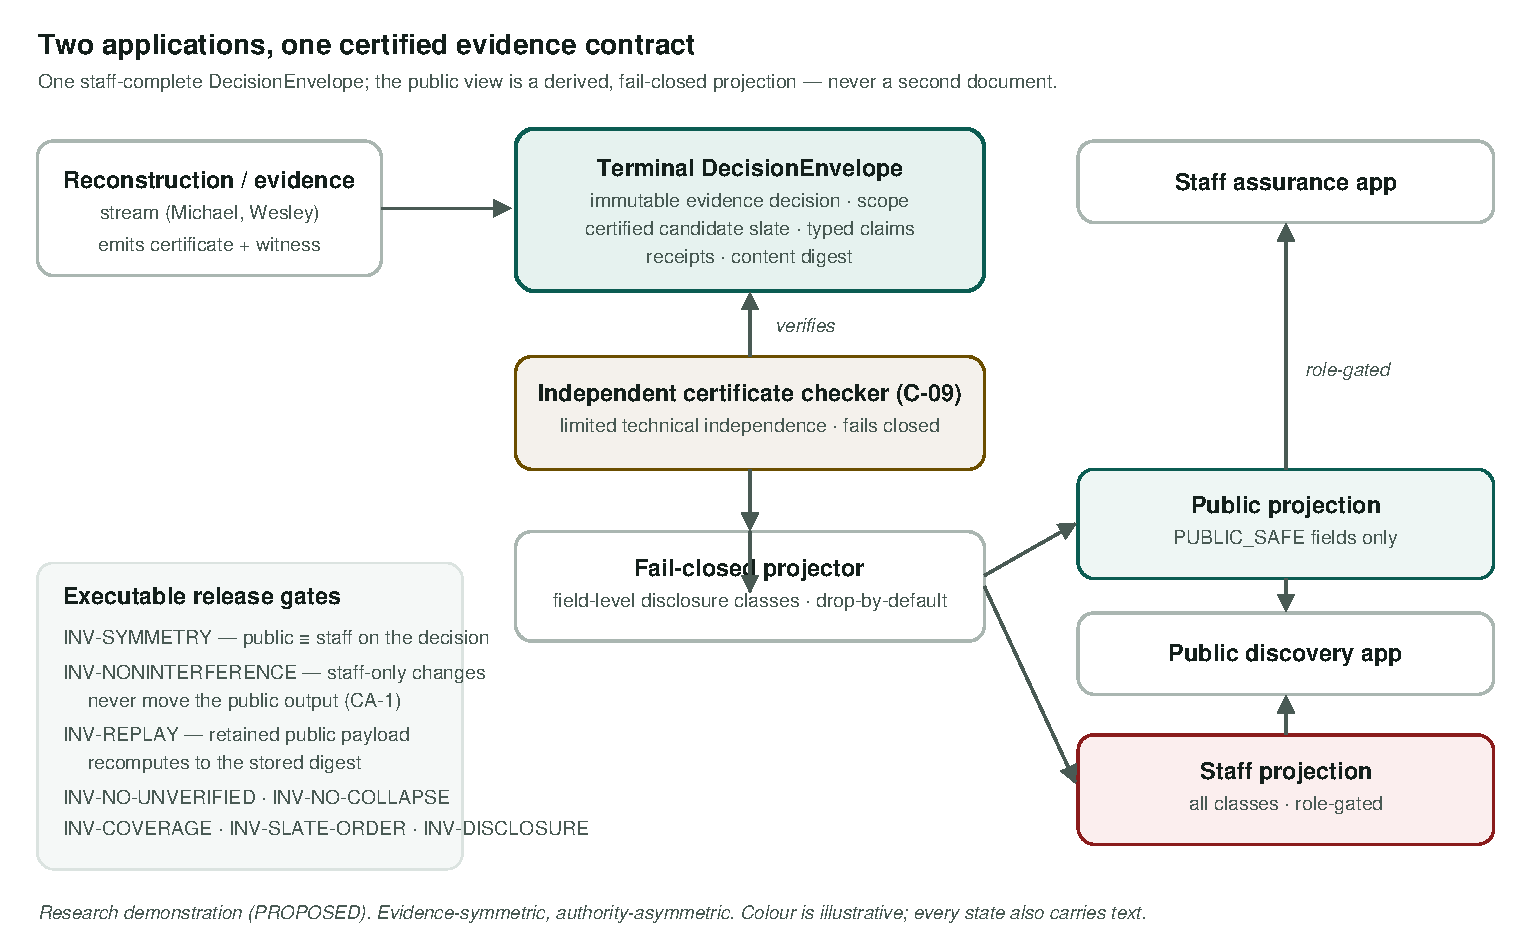
\includegraphics[width=\linewidth]{architecture-two-projections.pdf}
  \caption{One certified evidence contract, two permission-separated projections. A single terminal
  \texttt{DecisionEnvelope} carries the decision, scope, certified slate, claims and receipts; an
  independent checker verifies it; and a fail-closed projector derives a \textsc{public\_safe} public
  view and a role-gated staff view. Eight executable invariants act as release gates between them.}
  \label{fig:arch}
\end{figure}


% ####################################################################
% TABLE 1  —  PASTE INTO §3.2  (near "Table 1 sets out ...")
% IN-TEXT: replace "Table 1" with   Table~\ref{tab:checker}
% ####################################################################
\begin{table}[t]
\centering
\caption{Independent certificate checker (C-09): each injected defect is rejected with its exact
outcome code. Branch-mutation testing additionally kills all eight decision branches (0 survivors);
a well-formed certificate returns \texttt{PASS}.}
\label{tab:checker}
\begin{tabular}{@{}rll@{}}
\toprule
\# & Injected defect & Checker outcome \\
\midrule
1 & Missing witness & \texttt{FAIL\_MISSING\_WITNESS} \\
2 & Truncated evidence path & \texttt{FAIL\_MISSING\_WITNESS} \\
3 & Swapped receipt & \texttt{FAIL\_DIGEST\_MISMATCH} \\
4 & Forged hash & \texttt{FAIL\_DIGEST\_MISMATCH} \\
5 & Stale vintage & \texttt{FAIL\_VERSION\_MISMATCH} \\
6 & Incompatible schema/interpretation version & \texttt{FAIL\_VERSION\_MISMATCH} \\
7 & \texttt{U}/\texttt{B} escalated to supported & \texttt{FAIL\_ILLEGAL\_ESCALATION} \\
8 & Scope qualifier dropped & \texttt{FAIL\_SCOPE\_INCONSISTENCY} \\
9 & Ineligible candidate in a supported slate & \texttt{FAIL\_ILLEGAL\_ESCALATION} \\
10 & Certificate for another query & \texttt{FAIL\_DIGEST\_MISMATCH} \\
11 & Predicate outside the certifiable fragment & \texttt{FAIL\_UNSUPPORTED\_FRAGMENT} \\
12 & Unresolved receipt & \texttt{FAIL\_UNRESOLVED\_RECEIPT} \\
13 & Duplicated / ambiguous identity & \texttt{FAIL\_MALFORMED} \\
\bottomrule
\end{tabular}
\end{table}


% ####################################################################
% TABLE 2  —  PASTE INTO §3.5  (staff roles)
% IN-TEXT: cite as   Table~\ref{tab:roles}
% NOTE: \checkmark needs \usepackage{amssymb} if it errors.
% ####################################################################
\begin{table}[t]
\centering
\caption{Staff role $\to$ capability matrix (C-06/C-07). Access is not granted merely for being staff;
review, approval and send are separated (WP \S8.5). An action card can only be \emph{sent} by an
authoriser, and review/approval cannot be skipped.}
\label{tab:roles}
\begin{tabular}{@{}lccc@{}}
\toprule
Capability & analyst & assurance & authoriser \\
\midrule
view    & \checkmark & \checkmark & \checkmark \\
triage  & \checkmark & \checkmark & --- \\
draft   & \checkmark & \checkmark & --- \\
review  & ---        & \checkmark & --- \\
approve & ---        & \checkmark & --- \\
send    & ---        & ---        & \checkmark \\
\bottomrule
\end{tabular}
\end{table}


% ####################################################################
% TABLE 3  —  PASTE INTO §3.6  (disclosure classes)
% IN-TEXT: cite as   Table~\ref{tab:disclosure}
% ####################################################################
\begin{table}[t]
\centering
\caption{Field-level disclosure classes (C-BLOCK-05). The public view keeps only \textsc{public\_safe}
fields; projection is fail-closed, so any unclassified field is dropped from every plane. Counts are
of classified fields in the current contract.}
\label{tab:disclosure}
\begin{tabular}{@{}llp{6.4cm}@{}}
\toprule
Class (\#) & Visible on & Representative fields \\
\midrule
\textsc{public\_safe} (48) & public, staff, research & terminal decision, scope qualifier, recommendation action, coverage statement, candidate id/rank/pool, predicate evidence-state/mechanism/grade, digest, vintage \\
\textsc{staff\_aggregate} (15) & staff, research & internal score, model/policy version, latency, coarsened origin, failed stage, unevaluated feeds \\
\textsc{staff\_evidence} (15) & staff, research & receipts (id, content digest), lineage note, why-not predicate/blocking state, claim verification \\
\textsc{research\_restricted} (5) & research only & episode id, trace id, editable-interpretation source span \\
\bottomrule
\end{tabular}
\end{table}


% ####################################################################
% TABLE 4  —  PASTE INTO §3.6  (invariants)
% IN-TEXT: cite as   Table~\ref{tab:invariants}
% ####################################################################
\begin{table}[t]
\centering
\caption{Executable release-blocking invariants (C-BLOCK-05). Two valid fixtures pass all gates; six
adversarial fixtures are each detected by their targeted gate --- a gate that cannot fail is not
evidence.}
\label{tab:invariants}
\begin{tabular}{@{}lp{8.2cm}@{}}
\toprule
Invariant & Guarantees \\
\midrule
\texttt{INV-DISCLOSURE} & The public projection contains only \textsc{public\_safe} fields (content-scanned, not just keys). \\
\texttt{INV-NONINTERFERENCE} & Mutating only non-public fields leaves the public projection byte-identical (binds CA-1). \\
\texttt{INV-SYMMETRY} & Public and staff agree on decision, scope, action, coverage, candidate id + order, and vintage. \\
\texttt{INV-REPLAY} & The retained public payload recomputes to the stored digest (semantic replay). \\
\texttt{INV-NO-UNVERIFIED} & No claim whose verification $\neq$ verified is renderable. \\
\texttt{INV-NO-COLLAPSE} & No definite listing claim is made over a \texttt{U}/\texttt{B} predicate. \\
\texttt{INV-COVERAGE} & Every bounded non-match carries a coverage qualifier. \\
\texttt{INV-SLATE-ORDER} & Array order equals certified rank; an authorised slate holds only supported candidates. \\
\bottomrule
\end{tabular}
\end{table}


% ####################################################################
% TABLE 5  —  PASTE INTO §3.6 or Chapter 4  (assurance case)
% IN-TEXT: cite as   Table~\ref{tab:assurance}
% NOTE: the Verdict column is the TRUE state from validate_assurance.py
%       (evidence green, human gates open). This honest "blocked" is the
%       defensible reading for a research demonstration — keep it as-is.
% ####################################################################
\begin{table}[t]
\centering
\caption{Executable assurance case (C-16): 15 claims, each linked to a live check. The graph is sound
and all linked evidence is green; every claim is honestly \textsc{blocked} pending a named non-author
review and authority decision --- the correct maturity state for a research demonstration.}
\label{tab:assurance}
\begin{tabular}{@{}llc@{}}
\toprule
Claim & Guarantee (abbreviated) & Verdict \\
\midrule
CL-1  & public/staff never disagree; restricted values can't move public output & blocked \\
CL-2  & unknown is never rendered as a negative fact & blocked \\
CL-3  & no unsupported factual token reaches a user & blocked \\
CL-4  & certified slate and order preserved; abstention not bypassed & blocked \\
CL-5  & restricted staff information cannot leak; access is role-gated & blocked \\
CL-6  & forged/stale/swapped/escalated evidence rejected by the checker & blocked \\
CL-7  & application effects not confounded with backend differences & blocked \\
CL-8  & governed actions can't skip review/approval; send needs a role & blocked \\
CL-9  & all pre-code reconciliation blockers dispositioned & blocked \\
CL-10 & evaluated \emph{toward} WCAG 2.2 AA within a tested matrix & blocked \\
CL-11 & telemetry transient-by-default; no raw utterance or exact location & blocked \\
CL-12 & every human-facing activity ethically gated with a fallback & blocked \\
CL-13 & app-facing injection/output controls; no committed secret & blocked \\
CL-14 & conversation converges on the certified decision; never decides truth & blocked \\
CL-15 & every load-bearing source attested to K7 & blocked \\
\bottomrule
\end{tabular}
\end{table}


% ####################################################################
% BIBLIOGRAPHY  —  ADD THESE 6 ENTRIES to your .bib file
% (skip any your Background chapter already cites; reuse those keys instead)
% ####################################################################
% @inproceedings{geifman2017selective, ...}   -> see execution-refs.bib
% @inproceedings{lewis2020rag, ...}
% @article{rashkin2023attribution, ...}
% @article{bucinca2021trust, ...}
% @inproceedings{power2012guidelines, ...}
% @misc{w3c2023wcag22, ...}
% The full entries are in docs/report-figures/execution-refs.bib — copy them in.
